\chapter{物理疑难杂症}
\section{真空态与绘景}
\section{轴子和伸缩子}\label{A.2}
文献里经常会碰到这俩概念,虽然是作为暗物质的候选者,应当是唯象的关注对象,但形式理论中也处处见他们的身影。
\subsection{轴子(Axion)}
为了解释轴子的概念,先介绍\textbf{强CP问题}。这首先要从QCD的手征反常说起,后面会用到其中建立起来的一些工具。

\subsection{轴子电动力学}

\subsection{伸缩子(Dilaton)}
不少人也把它翻译成胀子。
\section{费曼规则}
这一节我不想讨论任何有关费曼规则推导的问题,只是通过拉氏量看出费曼规则,重点在对常用费曼规则的整理。本节讨论的都是动量空间的费曼规则,也就是把顶点的动量守恒都已经积成$\delta$函数了,计算上大家都是用的动量空间,因为更方便。
\subsection{标量场和矢量场}
这部分的费曼规则是基操,非常简单没有任何需要多说的,除了复标量场,由于和费米子又点想,留到下一小节再进行讨论。整体的费曼规则见图\ref{fig.A.3.2}(不包含顶角)。
\begin{figure}[htbp]
	\centering
	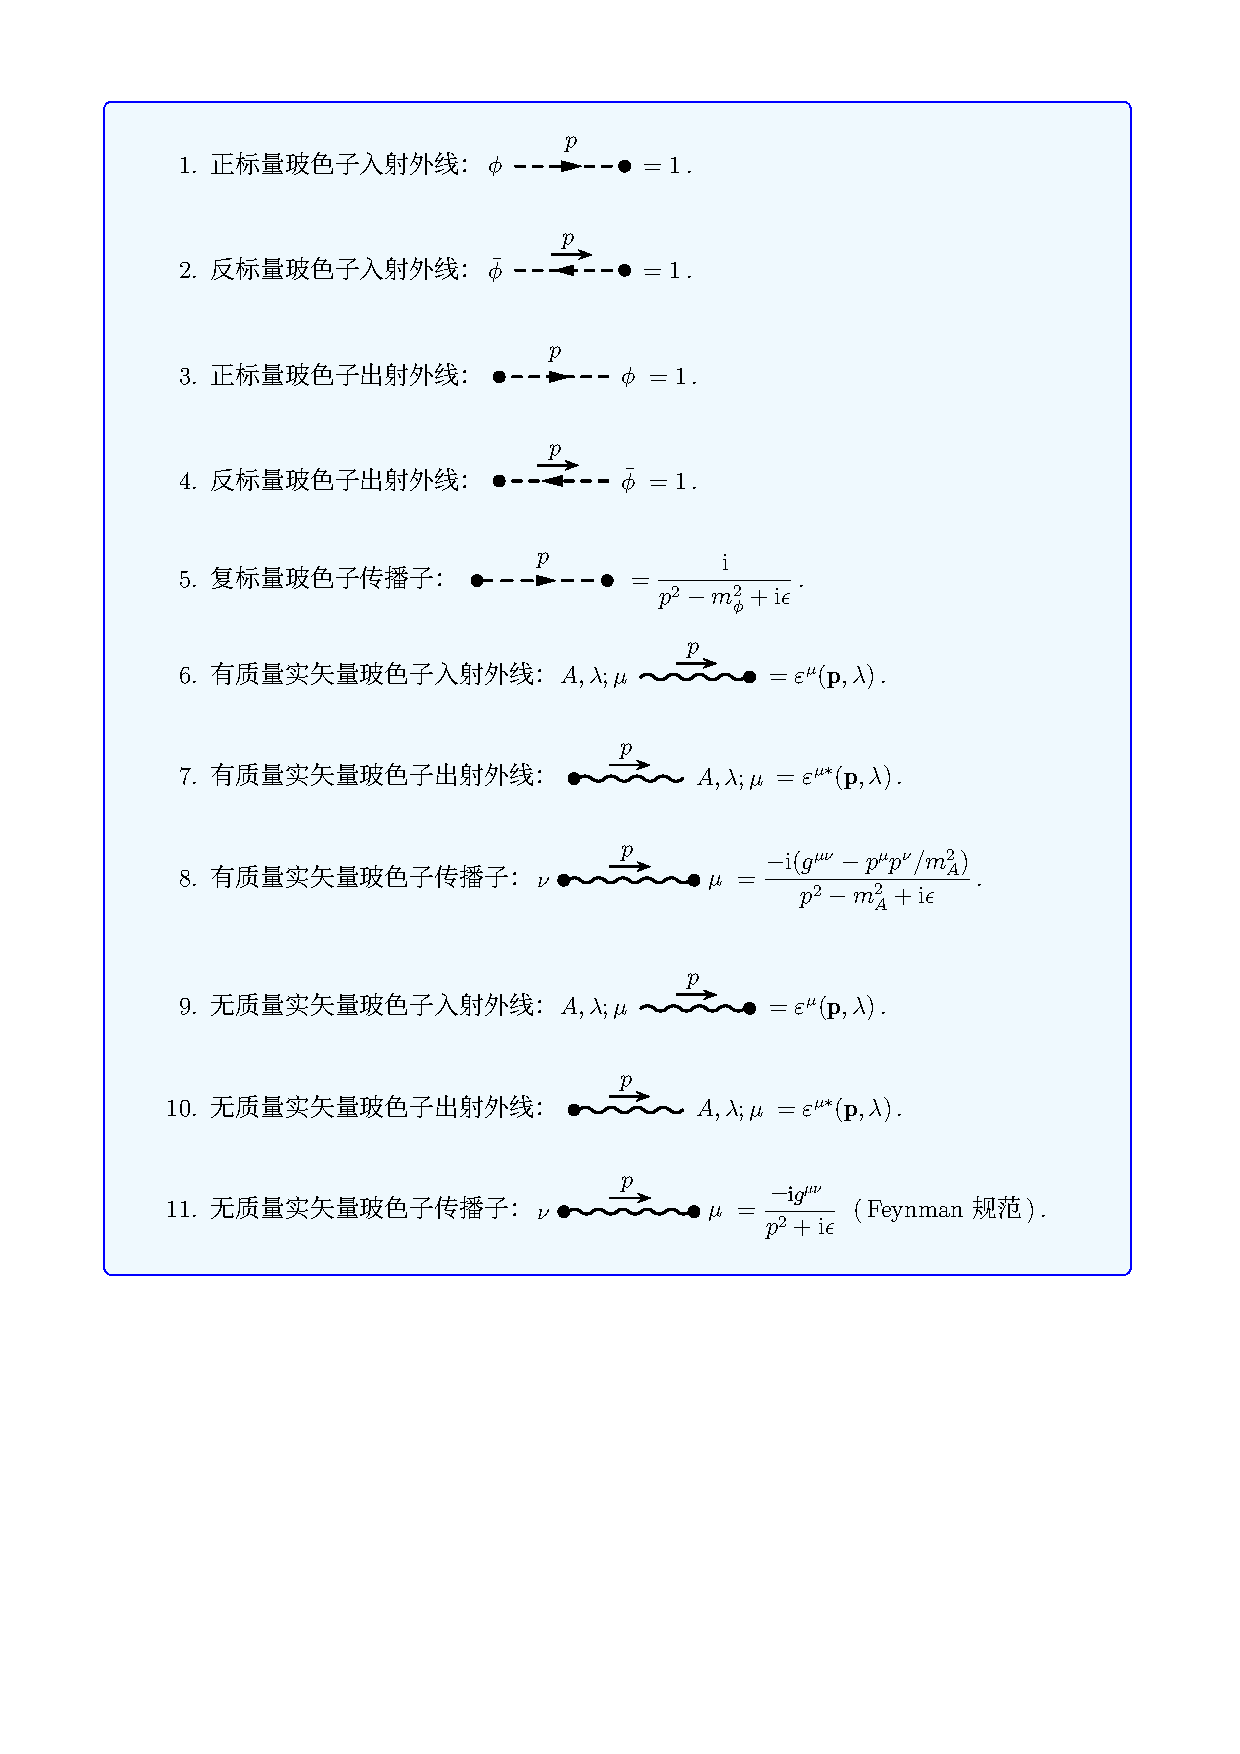
\includegraphics[width=\linewidth]{figs/fig20.pdf}
	\label{fig.A.3.2}
	\caption{一般内外线费曼规则}
\end{figure}
\subsection{Dirac和Majorana费米子}
这应该是费曼规则里最麻烦的部分,主要就是要分清三个箭头:动量箭头、$U(1)$箭头和费米子流箭头。很多教科书写费曼规则总是引入更少的箭头,反而搞一堆正负号规则,如果讨论的是标量场或者是矢量场,这没太大问题,但是对于旋量场,我认为最清楚的方式就是多画一些箭头。我们考虑下面的具有$CP$对称性的复标量场和Dirac场$\psi$以及Majorana场$\chi$的耦合:\footnote{这类费曼图构造可以更加复杂,尤其是涉及到费米子数破坏的理论。}
\begin{equation}\label{A.3.1}
	\mathcal{L}=(\partial^\mu\phi^\dagger)\partial_\mu\phi-m_\phi^2\phi^\dagger\phi+\bar{\psi}(\mathrm{i}\gamma^\mu\partial_\mu-m_\psi)\psi+\frac12\bar{\chi}(\mathrm{i}\gamma^\mu\partial_\mu-m_\chi)\chi+\mathcal{L}_\mathrm{int}
\end{equation}
从拉氏量可以看出我们选取的是$(+,-,-,-)$的度规\footnote{无论什么度规选取,都要保证对时间偏导的哪一个动能项是正的},原因是我本节费曼规则的图全部是抄的余钊焕老师讲义。这里相互作用项为:
\begin{equation}
	\mathcal{L}_\mathrm{int}=\kappa\phi^\dagger\bar{\chi}P_\mathrm{R}\psi+\kappa^*\phi\bar{\psi}P_\mathrm{L}\chi 
\end{equation}
选取$\kappa\in\mathbb{R}$,并引入记号$\Gamma_1=P_\mathrm{R},\quad\Gamma_2=P_\mathrm{L}$,这时为了突出下面的结果与$\Gamma_{1,2}$具体形式无关:
\begin{equation}
	\mathcal{L}_{\mathrm{int}}=\kappa(\phi^\dagger\bar{\chi}\Gamma_1\psi+\phi\bar{\psi}\Gamma_2\chi)
\end{equation}
其费曼规则如图\ref{fig.A.3.1}所示。下面我们来逐一解释每一项,并给出一些例子。
\begin{figure}[htbp]
	\centering
	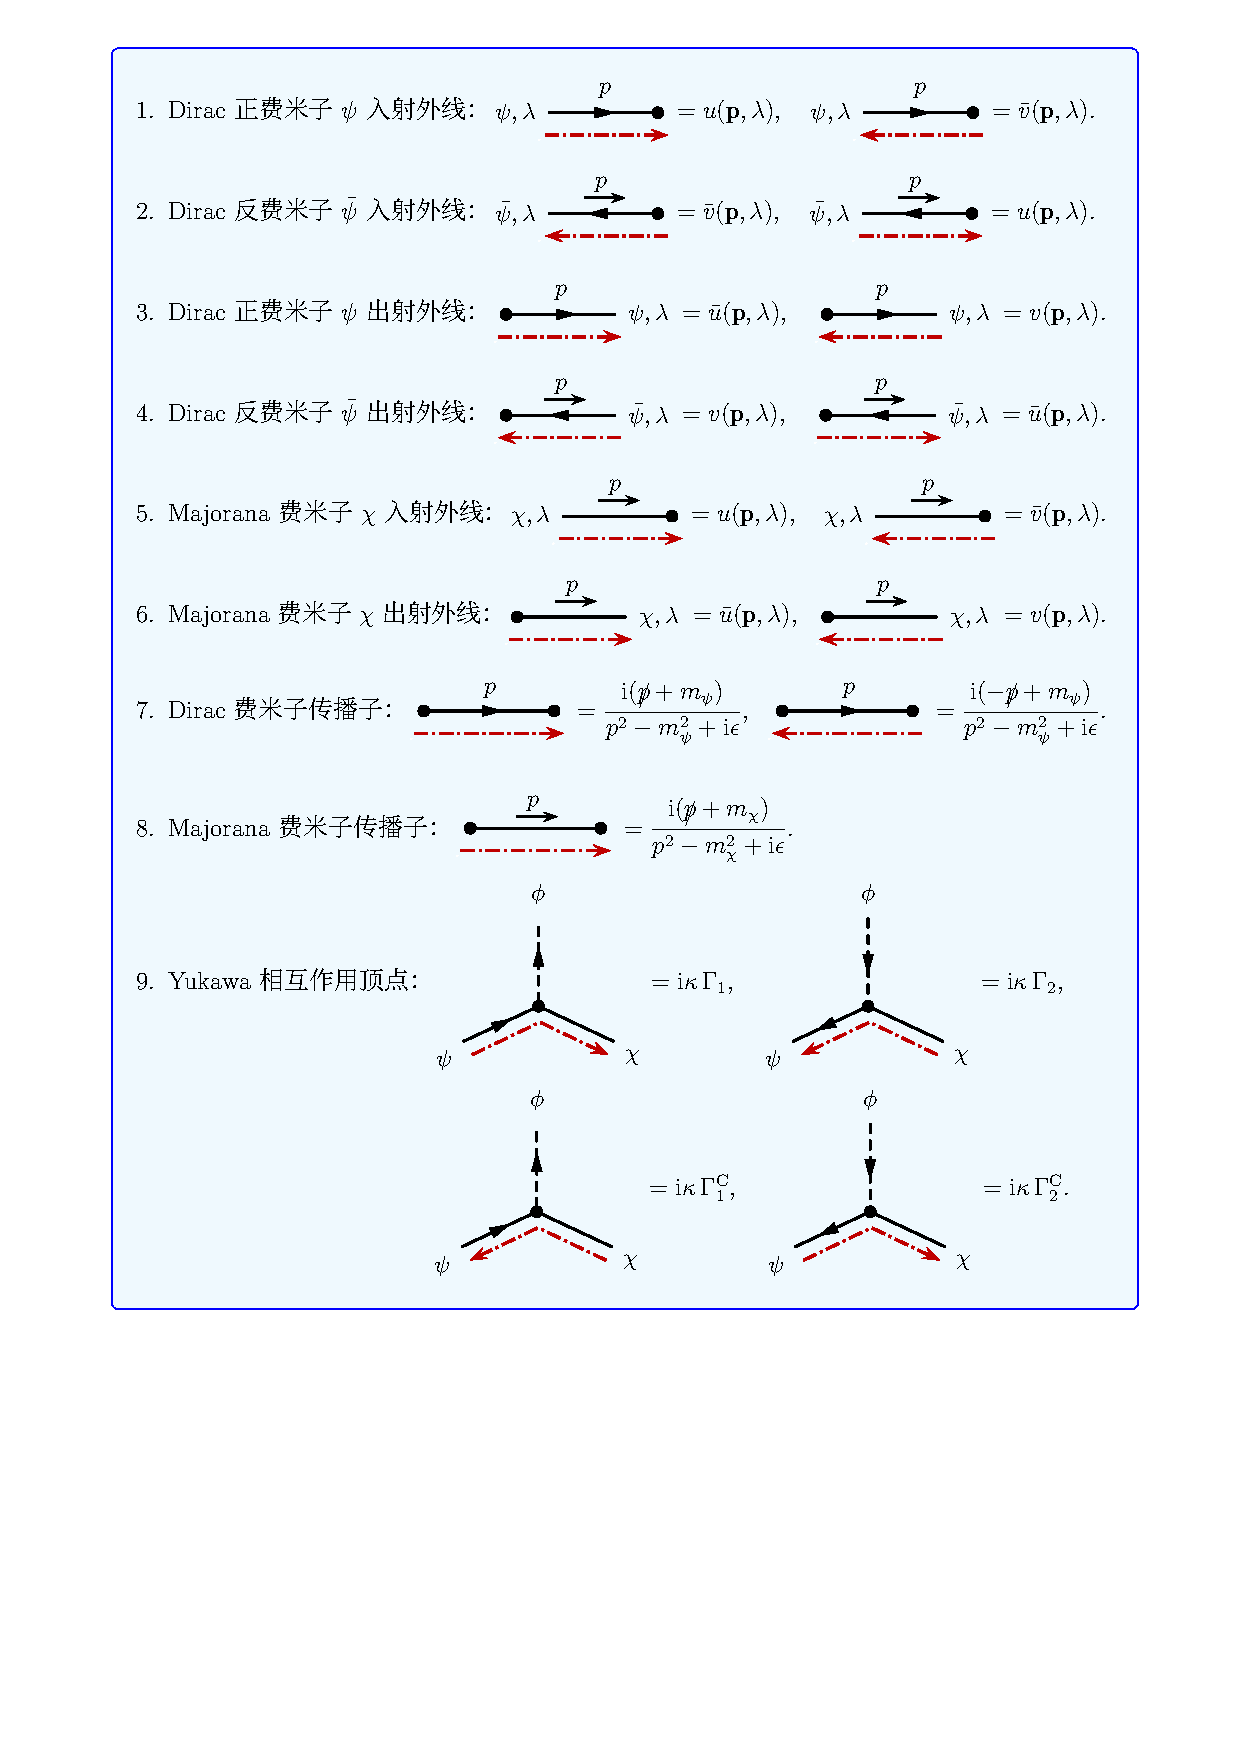
\includegraphics[width=\linewidth]{figs/fig19.pdf}
	\caption{\ref{A.3.1}的费曼规则}
	\label{fig.A.3.1}
\end{figure}

首先注意到图中出现了三种箭头,最上面的是动量箭头,标记的是粒子动量的正方向,根据这一点去要求每个顶点动量守恒,另外它还标记了粒子是入射还是出射,如果箭头流入节点,就是入射,流出就是出射;中间的是$U(1)$箭头,这是因为Dirac有正反两种不同的粒子所特有的,Majorana粒子就没有,这个箭头和动量箭头一起用来标记是正粒子还是反粒子,如果同向则为正,反向为反;最下面的箭头是费米子流,注意这个箭头是画在一整个费米子线段构成的折线上的,也就是说在每个费米子流线上,每个小段的流向一致,这是由于理论中有Majorana费米子,由于Majorana正反粒子相同,但是计算又必须引入一个方向所特别引入的一个附加规则。最后注意到有些图上我们把动量箭头和$U(1)$箭头合二为一了,这意味着两者是同向的,比如费米子内线我们就把两者取成一个方向。

再看顶角,这种复标量场和旋量场,根据耦合项读费曼规则,始终记住指向节点的表示$\phi\backslash\psi$,指出节点的是$\phi^{\dagger}\backslash\bar\psi$。Majorana耦合要根据费米子流来,复杂一点。复标量场的内外线规则可见\ref{fig.A.3.2},除了是玻色子,不需要引入费米子流来分清共轭、相对符号这些,其它和上一段讲的都一样。

另外我们这都是对树图的,对于圈图,还有一些来自圈的对称因子没有抵消殆尽,而且每个圈动量都要带来积分$\int\frac{d^4p}{(2\pi)^4}$,然后用维数正规化这些进行计算。而且\textbf{费米子圈会带来一个额外的符号},$\gamma$矩阵也要随之取迹。下面以$\chi\chi\to\psi\bar{\psi}$的计算为例。只考虑树图阶的贡献,首先第一步是根据费曼规则含有的顶点绘制出所有的不等价的费曼图,如图\ref{fig.A.3.3}
\begin{figure}[htbp]
	\centering
	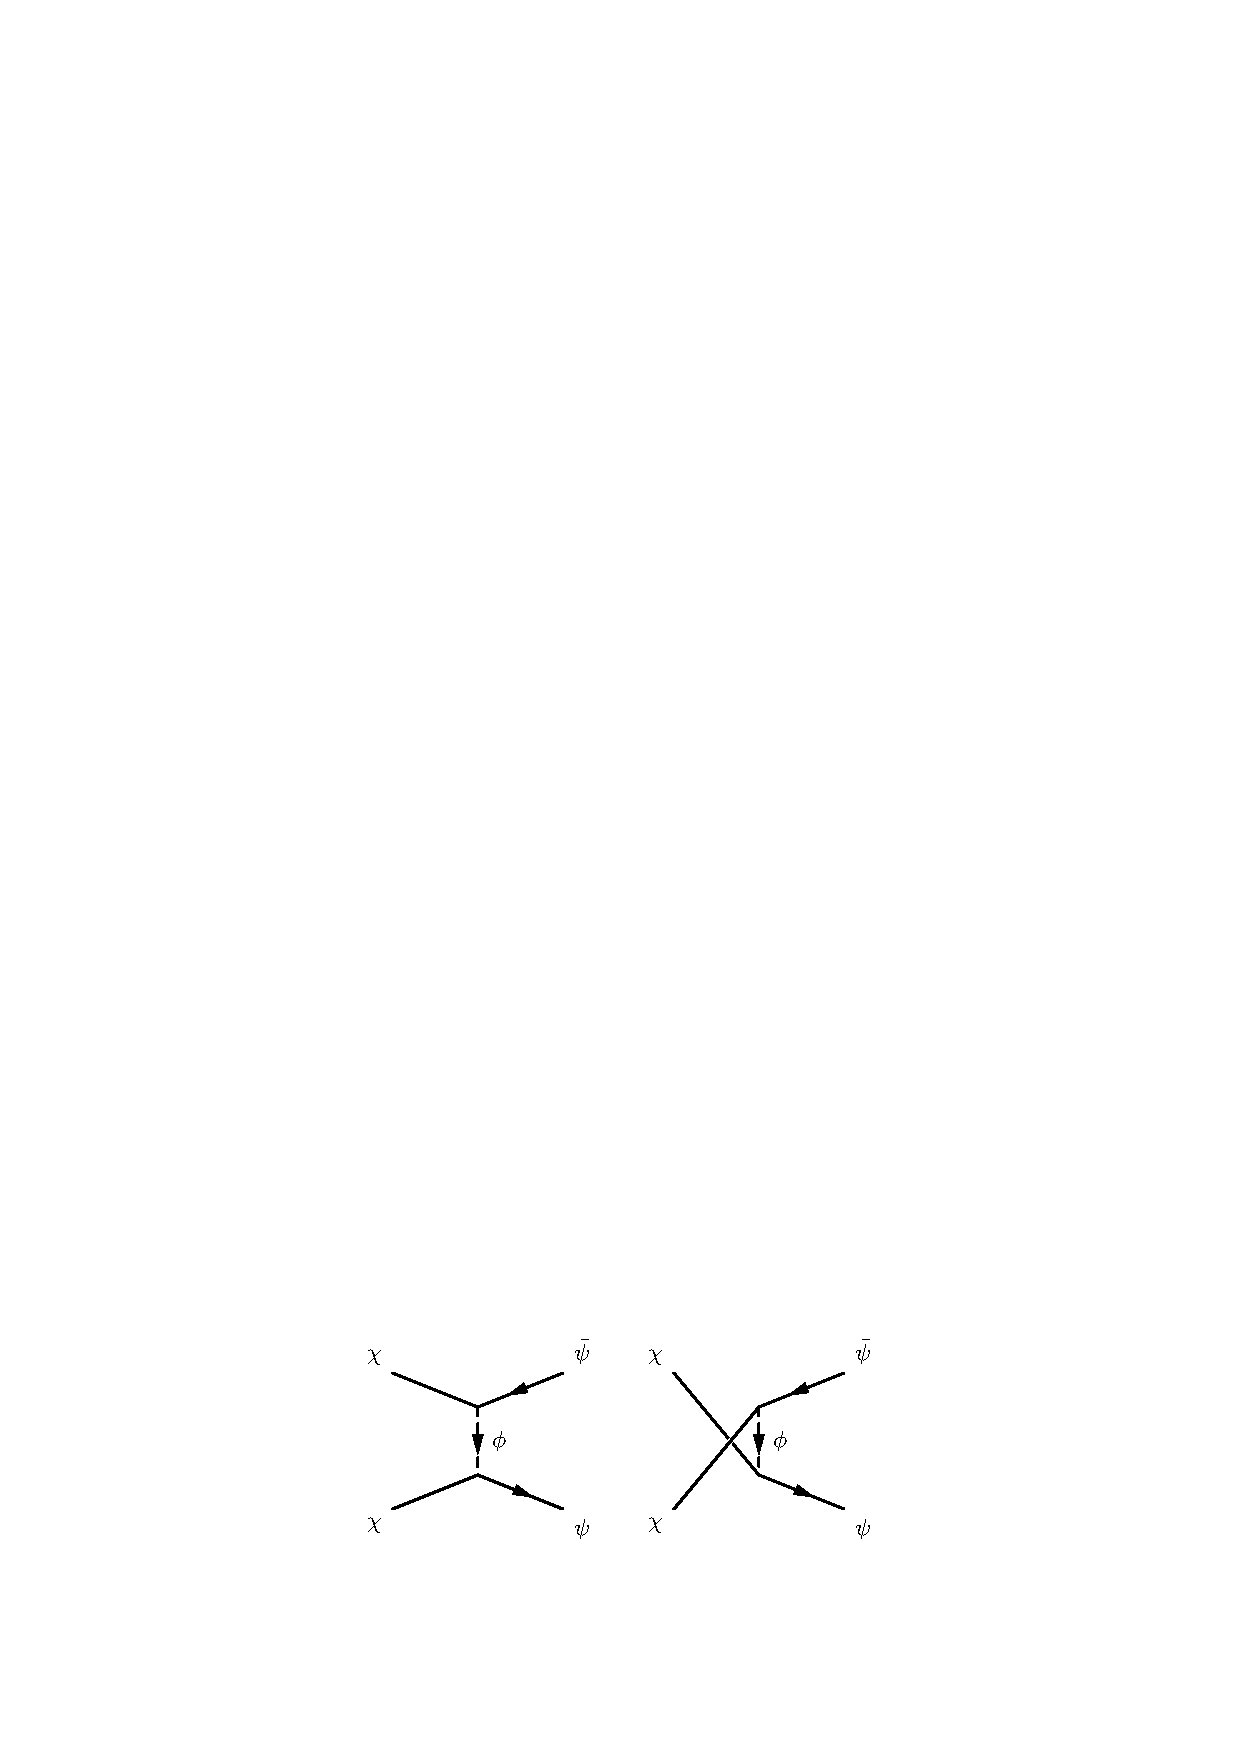
\includegraphics{figs/fig21.pdf}
	\caption{$\chi\chi\to\psi\bar{\psi}$散射树图}
	\label{fig.A.3.3}
\end{figure}

注意,我们并没有绘制费米子流,实际上图\ref{fig.A.3.2}给出的是两套等价的费曼规则,计算时我们需要人为地指定费米子流方向,然后逆着每个费米子流去写相应的项,无论怎么选费米子流,得到的结果都是一样的。比如下面的选取:
\begin{equation}
	\begin{aligned}
		\mathrm{i}\mathcal{A}_{t}&=\parbox[c]{3cm}{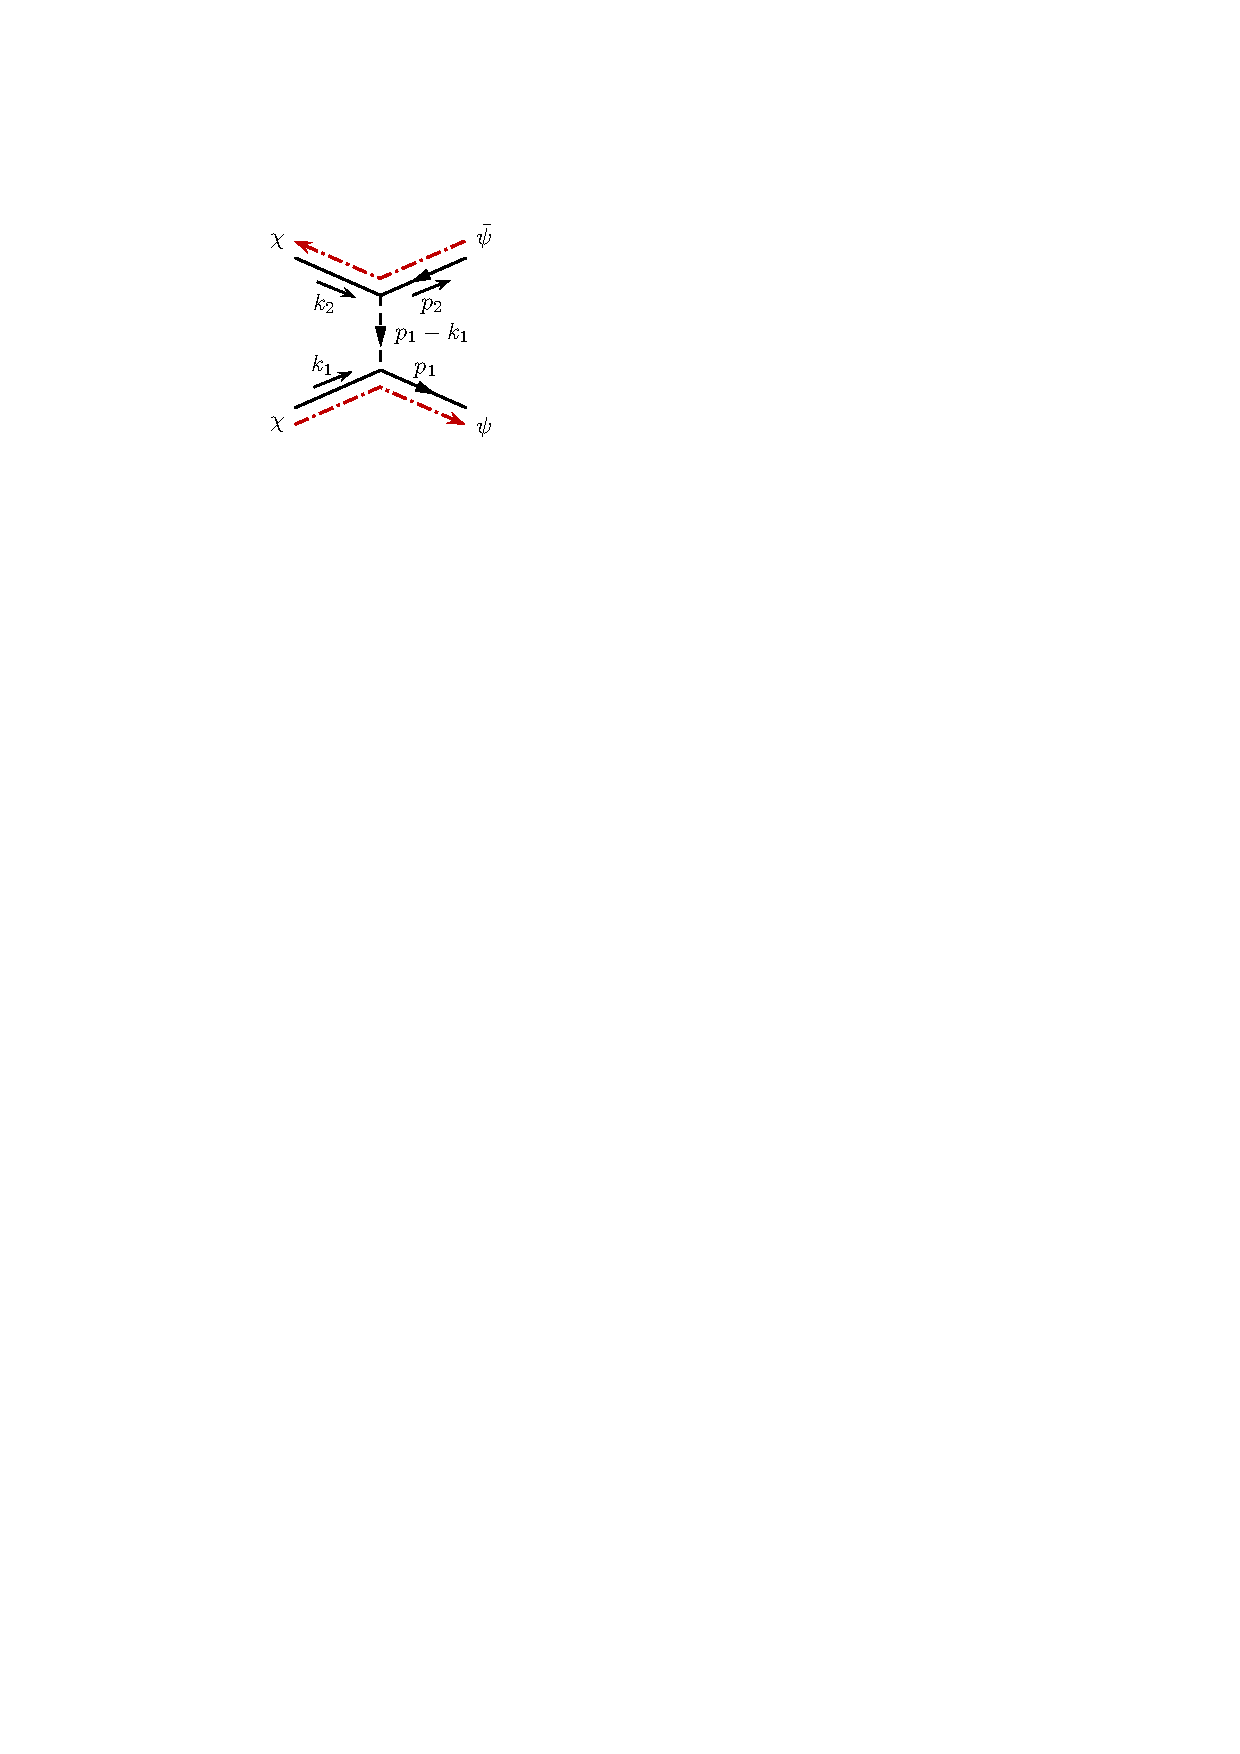
\includegraphics[width=3cm]{figs/fig22.pdf}}=\bar{u}(p_1)(\mathrm{i}\kappa\Gamma_2)u(k_1)\frac{\mathrm{i}}{(p_1-k_1)^2-m_\phi^2}\bar{v}(k_2)(\mathrm{i}\kappa\Gamma_1)v(p_2)\\
		&=-\frac{\mathrm{i}\kappa^2}{t-m_\phi^2}\bar{u}(p_1)\Gamma_2u(k_1)\bar{v}(k_2)\Gamma_1v(p_2)
	\end{aligned}
\end{equation}
\begin{equation}
	\begin{aligned}
		\mathrm{i}\mathcal{A}_{u}&=\parbox[c]{3cm}{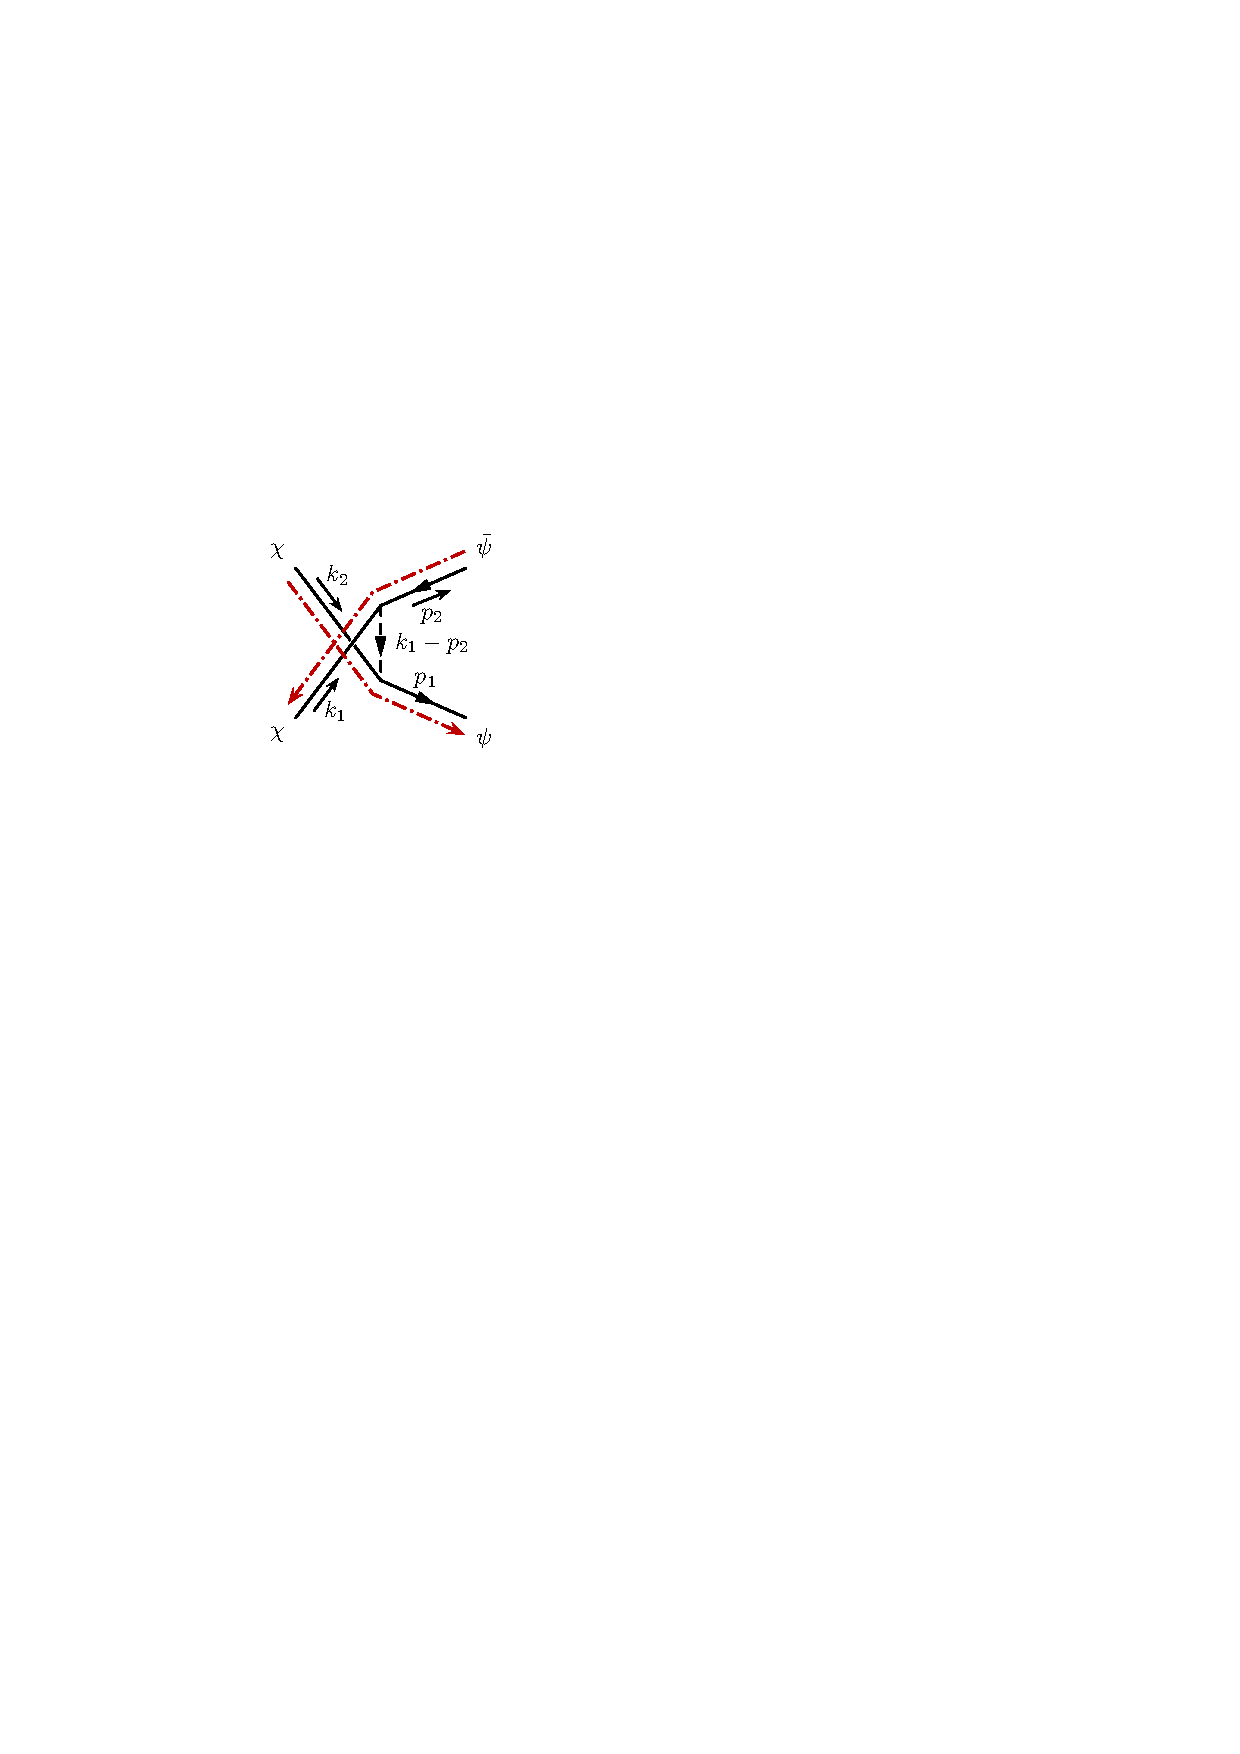
\includegraphics[width=3cm]{figs/fig23.pdf}}==\bar{v}(k_1)(\mathrm{i}\kappa\Gamma_1)v(p_2)\frac{\mathrm{i}}{(k_1-p_2)^2-m_\phi^2}\bar{u}(p_1)(\mathrm{i}\kappa\Gamma_2)u(k_2)\\
		&=-\frac{\mathrm{i}\kappa^2}{u-m_\phi^2}\bar{v}(k_1)\Gamma_1v(p_2)\bar{u}(p_1)\Gamma_2u(k_2)
	\end{aligned}
\end{equation}
费米子还有一个非常麻烦的地方就是不同费曼图贡献存在相对符号,如果一个过程只有一个图有贡献倒无所谓,但是多个图贡献就会导致干涉。这种符号的处理可以按照下面的规则:
\begin{description}
	\item[相对符号判断:]
\end{description}
所以容易判断上面的两项应该相减,$\mathrm{i}\mathcal{A}=\mathrm{i}\mathcal{A}_t-\mathrm{i}\mathcal{A}_u$。还有下面的费米子流选取方式:


对于只有Dirac旋量,不含Majorana旋量的费曼规则,上面的所有方法完全适用,只是这个时候就把费米子流取为和$U(1)$流同向,不用额外画出来。
\subsection{拉氏量顶点项中含有偏导数}
原则上所有的费曼规则的构造都可以回到路径积分或者正则量子化本身上去导出,我们不care这些原理,直接给结论怎么通过拉氏量看出来。